\chapter{绪论}
%
\section{研究背景和意义}
%
垂直领域检索增强对话生成任务有助于提高用户体验、解决特定领域的问题和提供个性化的服务。它可以应用于医疗保健、金融、法律、教育、科技等领域,为用户提供更加专业、全面和个性化的信息交流和服务。因此,垂直领域检索增强对话生成任务对于满足用户需求、提高工作效率、提供个性化服务等方面具有重要意义。

垂直领域检索增强对话生成目前主要的挑战是领域知识丰富,用户问题多种多样且抽象。针对领域知识丰富的挑战,研究人员致力于构建更加智能和灵活的对话生成模型,能够充分利用领域内的丰富知识资源,包括专业词汇、行业规范、学术研究成果等,以更好地应对用户的专业性问题。这包括基于知识图谱和预训练语言模型的技术,以及定制化的领域知识处理方法。针对用户问题多样性和抽象性的挑战,研究人员在探索如何构建更加灵活和多样化的对话生成模型,能够理解和回答各种类型的问题,包括事实性问题、推理性问题、情绪化问题\cite{JSJX202312001}等。此外,研究人员也致力于开发更加智能、个性化的对话交互方式,以满足用户多样化的沟通需求。同时,深度学习技术在对话生成任务中的应用也在不断演进。例如,针对领域知识丰富和用户问题多样性的挑战,研究人员正在探索如何通过多模态融合(如文本、图像、语音)、增强学习、迁移学习等技术手段,提高对话生成模型的适应性和泛化能力。

然而,相对于开放域对话生成,垂直领域对话背景知识更丰富,实现稳定、可控、准确的对话生成的技术挑战性更高,使垂直领域检索增强对话生成存在以下几个难点:

\begin{itemize}[topsep = 0 pt, itemsep= 0 pt, parsep=0pt, partopsep=0pt, leftmargin=36pt, itemindent=0pt, labelsep=6pt, listparindent=24pt]
	\item 难点1:内外部知识不一致问题。模型在预训练期间学习到的内部知识为常识知识,因此当模型迁移到垂直领域上时的泛化能力有限。现有方法大多关注如何提升外部知识召回准确度,而忽略了模型内部知识与之存在的分布差异,从而影响外部知识发挥作用,导致模型难以准确回答垂直领域专业问题。
	\item 难点2:人类偏好对齐问题。在垂直领域对话场景下,用户问题往往多样而复杂,模型难以从输入的用户问题中准确理解用户的真实意图,在语义检索和回答生成过程中存在数据分布偏差,导致模型生成不符合用户预期的回答。
\end{itemize}

近年来,越来越多研究人员投身面向垂直领域的检索增强对话生成研究\cite{RJXB202402009,DBLP:journals/corr/abs-2305-03653,DBLP:journals/corr/abs-2310-11511}。来自斯坦福大学、加利福尼亚大学、清华大学等国内外高校和企业研究机构的学者在该领域开展了大量研究工作\cite{DBLP:conf/emnlp/WangYW23,DBLP:journals/corr/abs-2306-16092}。国际上的一些主流学术会议和学术期刊也将垂直领域检索增强对话生成作为一个研究热点,如ACL、EMNLP等国际会议\cite{DBLP:conf/acl/ZhouZHHZ20,DBLP:conf/emnlp/JungSL20}。综上,面向垂直领域的检索增强对话生成研究是当前人工智能领域的重点与热点,不仅具有重要的理论价值,而且具有丰富的实际应用价值。

\section{本文主要研究内容}

\begin{figure}[htbp]
	\centering
	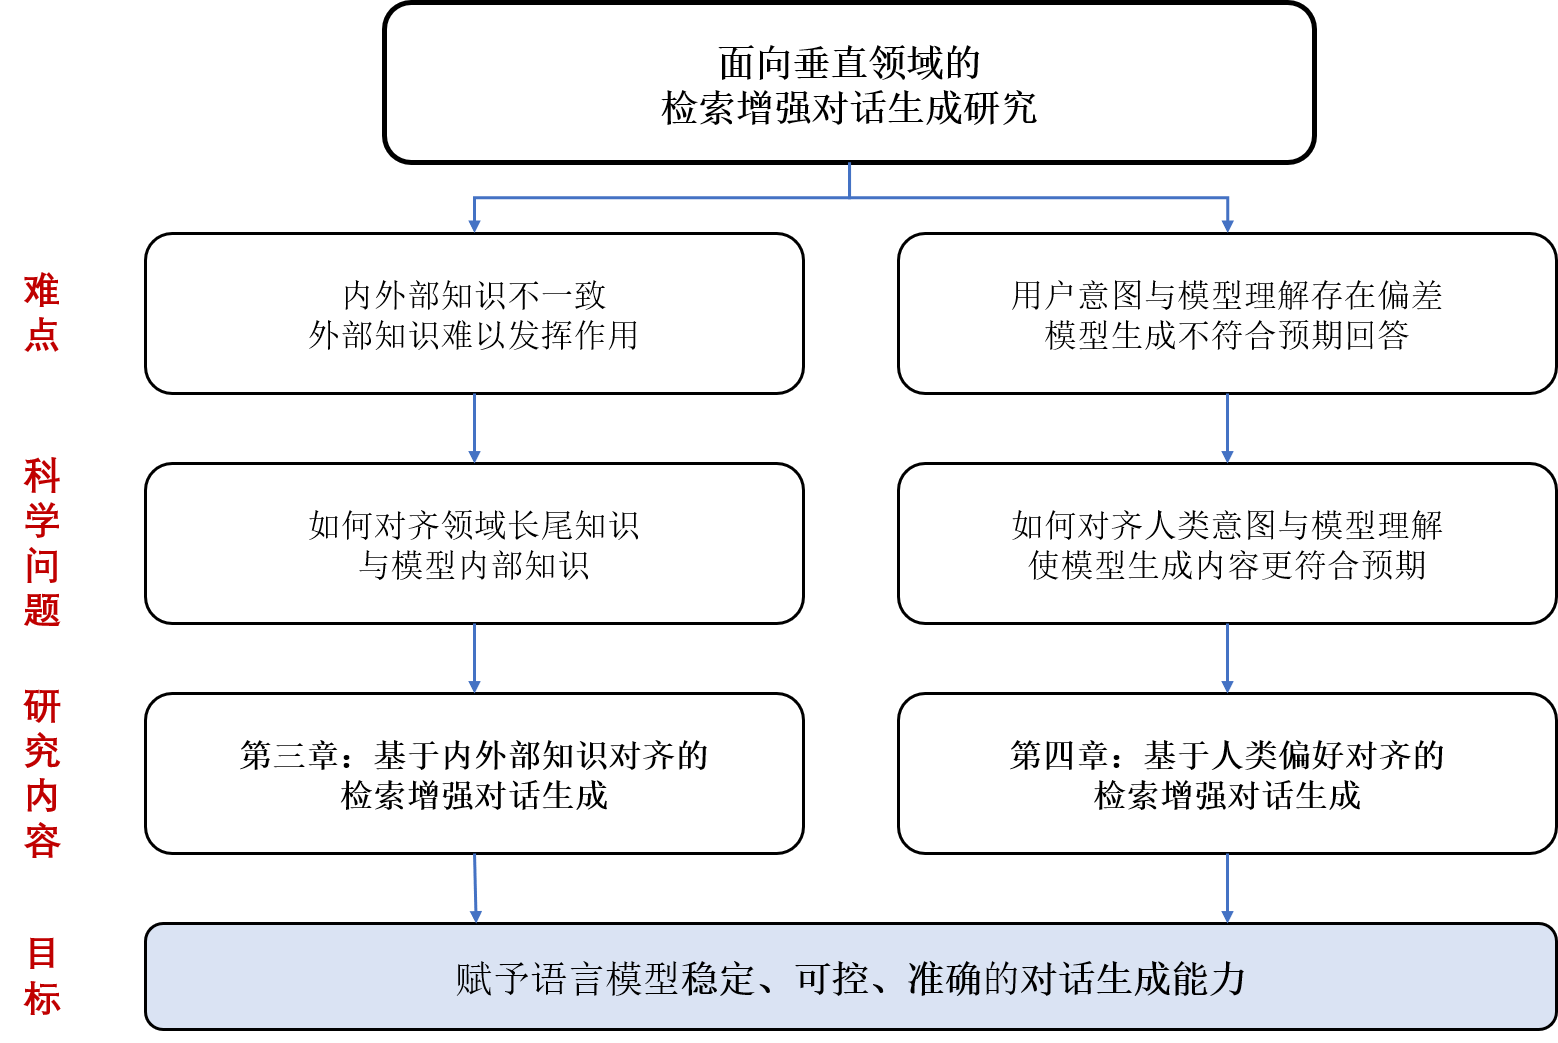
\includegraphics[scale=0.55]{Fig/paper_structure.png}
	\caption{\label{research_idea_and_research_content_of_this_paper}本文的研究思路与研究内容。}
\end{figure}

为解决上述挑战,本文主要研究在垂直领域场景下,如何利用对齐技术赋予语言模型稳定、可控、准确的对话生成能力,本文的研究思路与研究内容如图\ref{research_idea_and_research_content_of_this_paper}所示。包括基于内外部知识对齐的检索增强对话生成和基于人类偏好对齐的检索增强对话生成。本文的具体研究内容如下:

\begin{enumerate}[topsep = 0 pt, itemsep= 0 pt, parsep=0pt, partopsep=0pt, leftmargin=0pt, itemindent=44pt, labelsep=6pt, listparindent=24pt, label=\arabic*)]
	\item 基于内外部知识对齐的检索增强对话生成
	
	垂直领域知识背景复杂,语言模型在预训练中学习到的内部知识主要是常识知识,难以直接应用到垂直领域上做长尾问答,现有方法主要通过检索与用户问题相关的外部知识作为额外信息补充到模型输入中,然而,模型内部知识与外部知识之间存在较大分布差异,因此垂直领域外部知识难以发挥作用。针对上述问题,本文提出基于内外部知识对齐的检索增强对话生成方法,首先利用一个多粒度语义切分模块,从垂直领域知识文档中提取出文档级信息和实体级信息,并将提取出来的信息分别用于构建外部知识库和监督训练数据集,最后使用知识对齐后的数据集微调对话模型,有效避免了模型在预训练阶段注入的内部知识与推理阶段获得的外部知识不一致的问题。另外,本文结合知识库文档数量大、专有名词多的特点,提出关键词检索与向量检索相结合的多级检索模块,提升知识文档的召回准确率,进而提升对话生成的准确性。本文将该方法应用于金融、云计算和法律领域,在知识问答任务和金融领域真实股票趋势预测任务上验证了该方法的有效性。

	\item 基于人类偏好对齐的检索增强对话生成
	
	垂直领域对话场景下的用户问题往往多样而复杂,模型难以从输入的用户问题中准确理解用户的真实意图,在语义检索和回答生成过程中存在数据分布偏差,导致模型生成不符合用户预期的回答。另一方面,基于强化学习的人类偏好对齐算法训练成本高、稳定性差,使得对齐学习难度加深。针对上述问题,本文提出基于人类偏好对齐的检索增强对话生成方法,首先通过采集人类对真实场景对话样本的偏好信息,并利用大型语言模型的推理与分析能力进行用户问题优化,构成优化问题三元组数据集,用以训练单独的用户问题优化器,而无需训练对话模型,实现了与模型无关的、可解释、效果稳定的人类偏好对齐。本文分别在两个公开的金融基准测试集上与目前主流的语言模型对齐方法进行实验比较,证明了该方法的有效性。
\end{enumerate}

综上所述,本文的主要贡献包括:

\begin{enumerate}[topsep = 0 pt, itemsep= 0 pt, parsep=0pt, partopsep=0pt, leftmargin=0pt, itemindent=44pt, labelsep=6pt, listparindent=24pt, label=\arabic*)]
	\item 针对内外部知识不一致的问题,提出基于内外部知识对齐的检索增强对话生成方法,通过对齐内外部数据分布,提升模型对垂直领域外部知识的分析与理解能力;
	\item 针对人类意图与模型理解存在偏差的问题,提出基于人类偏好对齐的检索增强对话生成方法,通过对用户问题进行自动优化,提升外部知识文档召回的准确率和模型回复的质量;
	\item 在知识问答对话生成任务的数据集上进行实验,通过对比其他现有方法,以及对各模块进行消融实验,证明了本文所提出方法的有效性。
\end{enumerate}

\section{本文组织结构}

本文的组织结构和章节关系安排如下:

第一章是绪论部分,介绍了本文的研究背景与意义,分析了该研究方向的国内外研究现状,最后阐释了本文主要的研究内容和贡献。

第二章是对话生成研究现状,概述了与对话生成相关的国内外工作研究现状,包括对话系统的发展及相关工作,对面向垂直领域的对话生成主流方法进行梳理,以及对基于大型语言模型的对话生成方法进行总结和概述。

第三章提出了一种基于内外部知识对齐的垂直领域对话生成方法,利用一个语义切分模块提取知识文档的文档级信息和实体级信息,并将提取出来的知识分别用于构建外部知识库和内部知识注入,实现垂直领域对话模型内外部知识对齐。相关研究成果已经发表于自然语言处理和计算语言学领域的顶级会议COLING。

第四章提出了一种基于人类偏好的对话生成对齐方法,通过采集人类对真实场景对话样本的偏好,利用大型语言模型的理解与分析能力进行问题优化,并训练单独的问题优化语言模型,实现与模型无关的、可解释、效果稳定的人类偏好对齐。

第五章对全文研究工作进行了总结,并对领域未来研究方向进行了展望。
